% !TeX root = document-en.tex

\chapter{Introduction}
\label{chap:intro}

\makeendnotes  %make notes at the last of this chapter // if you do not  want use endnotes style, please comment out this.

\section{Organic semiconductors}

\subsection{Background}

For the past century, inorganic materials have been at the heart of the semiconductor industry, with element such as silicon, germanium or gallium arsenide. But the industry turned itself to new devices, and organics semiconductor are one of them. Their different set of properties: very flexible, low cost, less polluting helped them to gain more interest.

In 1977, the first highly conducting polymer was discovered: chemically doped polyacetylene \cite{polyacetylene}. Such material can be easily processed by techniques already know in the industry: vacuum evaporation, solution casting\dots But a better understanding and control of the self-assembly of molecules, as well as a booming research field, have greatly increased the performances, reaching the charge carrier mobility of amorphous silicon for some of them (fig. \ref{fig:1}). The high diversity of geometry within the material allows a better tuning of the characteristic of the semiconductor to the use cases. One greater advance is the combination of both organic and inorganic molecules, particularly with perovskite. The high mobility of inorganic material combined with the more flexible geometry of organic ones make possible the creation of devices that reaches the performances of single-crystal silicon \cite{IBM,perovskite}.

\begin{figure}
    \centering
    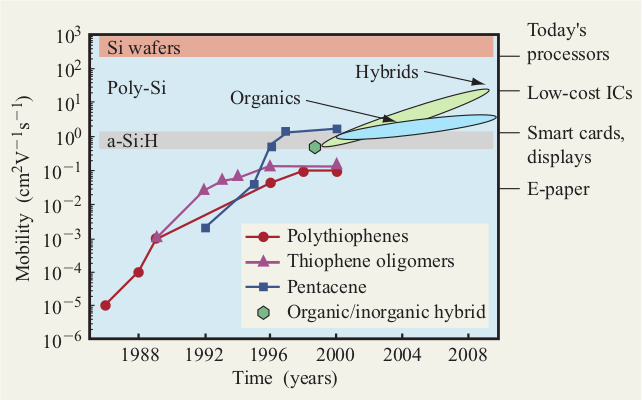
\includegraphics[width=.6\paperwidth]{figures/evolution_perf.png}
    \caption{History of the evolution of mobility in organic semiconductors \label{fig:1}\cite{IBM}}
\end{figure}

This new development has been seen through the recent appearance of organic devices in the market. The more flagrant one is OLED devices, they offer a better usability (flexible screens) with increased performance (higher color fidelity, darker black and better contrast) better electric consumption. It's also used in professional devices such as OTFT \cite{OTFT}, laser diode \cite{laserDiode}, \dots

\subsection{Future development}

Organic semiconductor are overwhelmingly used in wearable and portable devices, mainly as screen using thin-films transistors. They offer an affordable, biodegradable, transparent, flexible alternative to the classic inorganic TFTs. However, one key characteristic for such device is the transit frequency, the highest frequency at which we can operate the transistor. Most organic material have a frequency of at most a few mega-hertz, which is not enough for modern devices which works at the gigahertz frequencies. Usually, higher operating frequency means a higher quality final product. Replacing inorganic TFTs by organic one could mean a lot for the industry as both p-channel and n-channel can be fabricated at room temperature. But the increase in performance as recently stalled and need further development and research to really reach the performances of the more classical inorganic semiconductors \cite{frequency}.

\subsection{Organic materials}

Organic molecule are bound to each other by $\pi - \pi$ bounding which are the result of $p_z$-orbitals of $sp^2$-hybridized C-atoms in the molecules (fig. \ref{fig:2}). Such bonding is way weaker compared to the classic $\sigma$-bounding in the molecule backbone. Therefore, the $\pi-\pi^*$ transitions have a typical lower gap: around $\SI{1.5}{eV}-\SI{3}{eV}$ (fig. \ref{fig:3}). Their crystallinity ranges from single-crystal (pentacene, rubrene crystals) \cite{mono_crystal} to completely amorphous semiconductors like $\alpha$-NPD \cite{amorphous}.

\begin{figure}
    \centering
    \includegraphics*[width=0.4\paperwidth]{figures/pi_bonding.png}
    \caption{$\sigma$ and $\pi$ bonds in ethene \label{fig:2} \cite{intro_orga}}
\end{figure}

\begin{figure}
    \centering
    \includegraphics*[width=0.4\paperwidth]{figures/pi_pistar.png}
    \caption{$\pi-\pi^*$ bonding \label{fig:3} \cite{intro_orga}}
\end{figure}

Those weaker Van der Waals bonding lead to more localized charge carrier in the material. Most of the time, charge carriers do not evolve in bands like in Si, but are subject to a HOMO (Highest Occupied Molecular Orbital) and LUMO (Lowest Unoccupied Molecular Orbital) states. It results in a much weaker wavefunction delocalization for the neighboring molecules \cite{intro_orga}. Instead of band transport, organic materials are subject to hopping transport: a charge carrier hop from a site to an other and thus participate to the general conduction (fig.\ref{fig:4}). The difference between trapping and hopping state is in the recombination and release rate. if the former one is higher than the letter one, the state is a recombination center, otherwise, it is a trap. In this model the difference between trapping states and recombination states can be thin.

\begin{figure}
    \centering
    \includegraphics*[width=0.4\paperwidth]{figures/hopping_theory.png}
    \caption{Hopping transport \label{fig:4}}
\end{figure}

Organic semiconductors are divided between polymers and small molecules. The separation occurs at $1000$ molecular weights. Small molecules can achieve high cristallinty but are less soluble in solvent, requiring dry processes such as vacuum deposit, which is more difficult and more costly. On the other hand, polymer are easier to made in organic solvents. Even though small molecules show better performances, they're less stable than polymer in atmospheric conditions.

\subsection{Charge carrier transport}

As it has been said before, disorganized organic semiconductors are the place of localized charge carrier transport, and in the 70's, a theory has been proposed involving tunneling between near states \cite{hopping_theory_1}. Such theory as been previously discovered by Mott based on the dependence of the mobility on the temperature: an increasing temperature leads to an increasing mobility. This relation has been verified in practical devices \cite{hopping_theory_1,multiple_theory}.

In the variable range hopping theory (VRH), the displacement between two states for a charge carrier is determined only by the difference in energy $W$ and in position $R$, thus highlighting the fact that our system is resolutely in 4D. On top of that, we assume that the system is so disordered that this two quantities are decoupled. The jump frequency is usually described by the Miller-Abrahams formalism \cite{miller}:

\begin{equation}
    \nu=\nu_{0}\left\{\begin{array}{r}
    \exp \left(-2 \alpha R_{i j}-\frac{E_{j}-E_{i}}{k_{B} T}\right): E_{j}-E_{i} \geq 0 \\
    \exp \left(-2 \alpha R_{i j}\right): E_{j}-E_{i} \leq 0
    \end{array}\right.
    \label{eq:1}
\end{equation}

\begin{itemize}
    \setlength\itemsep{0.1em}
    \item $\nu_0$: base-jump frequency
    \item $R_{i j}$: distance between initial state $i$ and final state $j$
    \item $\alpha$: decay constant of the assumed hydrogen-like localized state wave functions
    \item $E_i$: energy of the state $i$
\end{itemize}

Depending on the position of the final state $j$, the formula changes. If the state is on higher energy, it requires tunneling to occur on the energetic part, whereas if the reaching state if of a lower energy, only the distance is taken into account for the tunneling effect, the jump being energetically favorable.

Using this formalism, it is possible to access the mobility and diffusivity for charge carrier.

\subsection{The Einstein relation}

It has been reported in organic semiconductor that the classical Einstein relation may be violated in certain conditions \cite{general_einstein}. To better understand the changes in the Einstein ratio, we will first present the classic equation before explaining what can change.

\subsubsection{Classical Einstein relation}

\begin{equation}
    \frac{D}{\mu} = \frac{k_bT}{q}
    \label{eq:2}
\end{equation}

\begin{itemize}
    \setlength\itemsep{0.0em}
    \item $\mu$: mobility
    \item $D$: diffusion
    \item $k_B$: Boltzmann constant
    \item $T$: temperature
    \item $q$: elementary charge
\end{itemize}

The Einstein relation \cite{Einstein}, is a useful equation that link two quantities, $\mu$ and $D$ over a simple equation. $D$ constitutes a key parameter in analyzing semiconductor but is not so easy to measure. On the contrary, the mobility is easily accessed. However, in the presence of energetic disorder, such simple equation does not seem to hold \cite{ein_drift,ein_drift_2}. In non-equelibrium cases, it also seems that we can't use this relation anymore, the relation between the diffusion and the field seems to be quadratic \cite{diffusion_F}.

\subsubsection{Generalized equation}

From the limit of the eq. \ref{eq:2}, a new relation has been proposed, taking into account the dependence on the carrier concentration \cite{generalied_quasi}:

\begin{equation}
    \frac{D}{\mu}=\frac{n}{q \partial n / \partial E_{F}}
    \label{eq:3}
\end{equation}

\begin{itemize}
    \setlength\itemsep{0.0em}
    \item $E_F$: quasi-Fermi level
    \item $n$: carrier concentration
\end{itemize}

With $n$ being the carrier concentration defined by the fermi-dirac distribution $f = \frac{1}{1 + exp\left(\frac{E - E_F}{k_BT}\right)}$ and $g$ the gaussian density of state \cite{generalied_quasi}:

\begin{equation}
    n=\int_{-\infty}^{\infty} \frac{g(E)}{1+\exp \left(\frac{E-E_{F}}{k_{B} T}\right)} d E
    \label{eq:4}
\end{equation}

Such eq. \ref{eq:4} has been calculated following the hypothesis that drift and diffusion of charge carrier at fermi level are exactly compensated, meaning that there is no net current and is only valid for low electric field.

From this stating, a more suitable equation has been proposed in the following thesis.

\subsection{Gaussian density of states}

\begin{equation}
    g(E)=\frac{N}{\sigma \sqrt{2 \pi}} \exp \left(-\frac{E^{2}}{2 \sigma^{2}}\right)
    \label{eq:5}
\end{equation}

Gaussian density of states has been suggested by numerous monte-carlo simuations \cite{DOS_monte_carlo} as well by the observation of the excitonic absorption profile which is gaussian too. Besides, the intrinsic localization behavior of the gaussian density of state fit very well the observation made on real devices.

From a mathematical point of view, the disorder is directly linked to $\sigma$, which broadens the bell-shaped function (fig. \ref{fig:5}, \ref{fig:6}).

\begin{figure}
    \centering
    \includegraphics*[width=.5\paperwidth]{figures/DOS_1.png}
    \caption{Gaussian DOS, $\sigma=1$ \label{fig:5}}
\end{figure}

\begin{figure}
    \centering
    \includegraphics*[width=.5\paperwidth]{figures/DOS_3.png}
    \caption{Gaussian DOS, $\sigma=3$ \label{fig:6}}
\end{figure}

\subsection{Thermal diffusion}

Organic semiconductors have recently received much attention regarding their potential thermoelectric effect. From their figure of merit (eq. \ref{eq:6})

\begin{equation}
    \mathrm{ZT}=\frac{\sigma \cdot S^{2}}{k} T
    \label{eq:6}
\end{equation}

\begin{itemize}
    \item $S$: Seebeck coefficient
    \item $\sigma$: electrical conductivity
    \item $k$: thermal conductivity
\end{itemize}

ZT value is representative of the device thermo-electric efficiency. A lower thermal conductivity $k$ naturally leads to higher figure of merit and to an increased energetic conversion.

A better understanding of the thermo-electric behavior is key to engineering better devices, but the classical theory used on inorganic material \cite{einstein_model_thermic} can't be applied directly to organic ones. The variety of morphology in organic semiconductors plays a great role in defining its thermal characteristics and is extremely sensitive to the spacial arrangement of the molecules within the material.

To simulate the thermal effect, one should take into account both charge carrier and phonon transport: $k = k_e + k_p$ with a slight predominance of the phonon in the process of thermal conduction \cite{universal_einstein}.

\section{Objectives of this thesis}

The overall understanding of both electric and thermal behavior of organic semiconductors is scarce. Their great diversity, which is at the heart of their recent success, makes it difficult to get an accurate simulation of the charge carrier in the material. The goal of this thesis is to obtain, thanks to equations developed throughout the 20th century and to new hypothesis on the comportment of the charge carrier, as well as a powerful computer language, a reasonable approximation of the electric and thermal figures in doped organic semiconductors:

\begin{itemize}
    \item Estimating Einstein ratio for many type of organic semiconductors
    \item Taking into account the doping behavior of the semiconductor, as well as the disorder and electric effect
    \item Estimating the thermal conduction by taking into account both charge carrier and phonon participation
    \item Simulating the model in a fairly small amount of time
\end{itemize}

The novelty of this study resides in the multitude of the parameters taken into account and in new behavior for charge carrier within the material.